\documentclass{beamer}
\beamertemplatenavigationsymbolsempty
\usepackage{amsmath, amssymb, hyperref, graphics}
\usepackage{graphicx}
\usepackage{tikz}
\usetikzlibrary{arrows}


\title{Graph Theory Lecture 10}

\begin{document}
\begin{frame}{The Travelling Salesperson Problem}
\begin{block}{Informally:}
  A Travelling Salesperson wants to start from home, visit every city on their list, then return home for as cheaply as possible.
\end{block}

\begin{definition}
The \emph{Travelling Salesperson Problem}, or TSP, is the following.  Given a weighted graph $G$ (usually $G$ is the complete graph), what is the Hamiltonian cycle (i.e. closed walk visit every vertex) of cheapest weight?
  \end{definition}

\begin{block}{The TSP is \emph{Hard}}
  \end{block}

\end{frame}

\begin{frame}{The TSP is at least as hard as finding Hamiltonian cycles}
  Let $G$ be a graph $n$ and vertex set $V$ and edge set $E$. \\
  Suppose we want to determine whether $G$ has a Hamiltonian cycle.\\
Weight a complete graph on the vertex set $V$ as follows: make every edge in $G$ have weight 1, and every edge \emph{not} in $G$ have slightly higher weight:
  $$w(uv)=\begin{cases} 1 & uv \in E \\
1+\varepsilon & uv\notin E\end{cases} $$
Then, $G$ has a Hamiltonian cycle if and only if there is a solution to the TSP with weight $n$.

\begin{block}{Bound the TSP instead of solving it}
  \end{block}
\end{frame}

\begin{frame}{Can \emph{almost} solve TSP in practice}
  Programs such as \emph{Concorde} use sophisticated ideas to get solutions to TSP within a few percentage points on large data sets.
  \begin{columns}
  \begin{column}{.5\textwidth}
\begin{center}    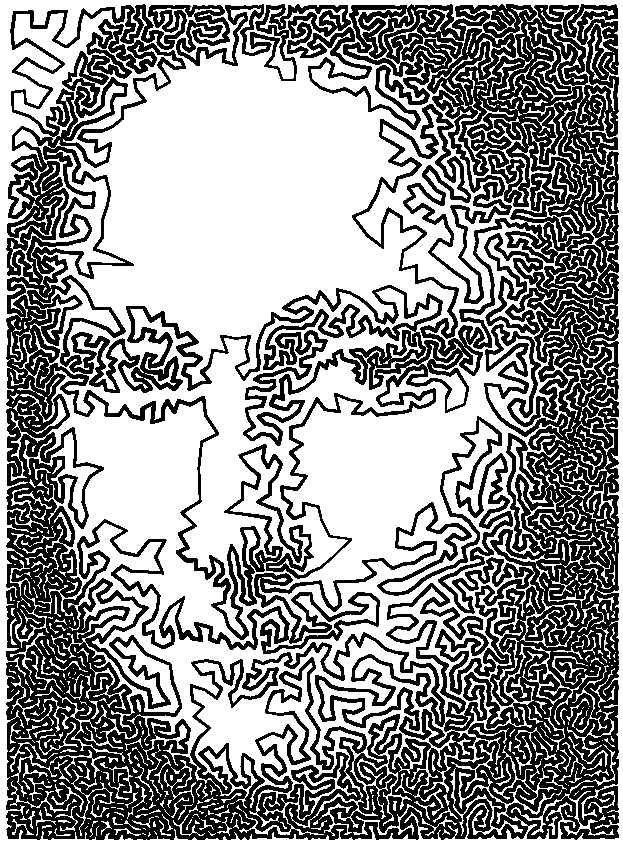
\includegraphics[scale=.5]{mona.pdf} \end{center}
  \end{column}
  \begin{column}{.5\textwidth}
\begin{center}
  From \emph{TSP Art} \\ \\ by\\ \\Craig S Kaplan \\ \\ and\\ \\Robert Bosch
  \end{center}
  \end{column}
  \end{columns}
\end{frame}

\begin{frame}{To get an upper bound on TSP, find the weight of any Hamiltonian cycle}
  \begin{block}{One greedy algorithm: nearest neighbour}
    Keeping going to the closest city you haven't been to
  \end{block}
  \begin{block}{Why might nearest neighbour be bad?}
  \end{block}

  \begin{block}{Better heuristics exist:}
    \begin{itemize}
    \item Nearest insertion: grow loop by inserting nearest city
    \item Christofide's Algorithm finds a Hamiltonian cycle at most 3/2 as expensive as the cheapest
    \end{itemize}
    These are more involved than nearest neighbour and still don't solve problem
    \end{block}
  \end{frame}

\begin{frame}{To get a lower bound on TSP, can't use a cycle}
  Any Hamiltonian cycle has length \emph{greater} than solution to TSP.
  \begin{block}{To find lower bound to TSP}
    \begin{itemize}
    \item Pick a vertex $v\in G$
    \item Find a minimum weight spanning tree $T$ on $G\setminus v$
    \item Find the two cheapest edges $e_1$ and $e_2$ out of $v$
    \item $w(T)+w(e_1)+w(e_2)$ is a lower bound
    \end{itemize}
    \end{block}

  \begin{block}{Need to be able to prove this gives lower bound...}
  \end{block}
  
  \end{frame}

\begin{frame}{Prove that $w(T)+w(e)+w(f)\leq TSP$}
  Suppose that $C$ was the Hamiltonian cycle of minimum weight.  We split the $C$ into two pieces: the two edges $f_1$ and $f_2$ adjacent to $v$, and the rest, which we'll call $R$.

 \begin{block}{Edges adjacent to $v$:}
   $e_1$ and $e_2$ were the two cheapest edges next to $v$, so:
   $$w(f_1)+w(f_2)\geq w(e_1)+w(e_2)$$
 \end{block}

 \begin{block}{The rest:}
\begin{itemize}
\item $C$ a cycle, so $R=C\setminus v$ is a path
\item Paths are special cases of trees
\item $R$ visits every vertex of $G\setminus v$
\item Hence $R$ a spanning tree and $w(R)\geq w(T)$
  \end{itemize}
 \end{block}
 \end{frame}
\begin{frame}{Example from the 2006 Exam}
  The following table encodes distances between towns in km:
$$
  \begin{tabular}{ccccccc}
    A   &   &   &   &   &   & \\
    23  & B &   &   &   &   & \\
    10  & 21& C &   &   &   & \\
    30  & 39& 21& D &   &   & \\
    57  & 45& 48& 45& E &   & \\
    68  & 63& 59& 47& 24& F & \\
    75  & 67& 66& 54& 24& 11& G
    \end{tabular}
  $$
  Find lower and upper bounds to the TSP.

  
\end{frame}
  






\end{document}
